\section{The Simplex Method}
\label{sect:simplex-method}
\begin{enumerate}
\item In \labelcref{it:reduce-to-std-form}, we have mentioned that algorithms
are available for solving \emph{standard form} LP problems. A popular one is
the \emph{simplex method}, which is the main topic to be discussed in
\Cref{sect:simplex-method}. Throughout we shall focus on standard form LP
problems.
\end{enumerate}
\subsection{Optimality Conditions}
\begin{enumerate}
\item The concept of \emph{optimality conditions} is critical for the simplex
method and also many other optimization algorithms. Indeed, to
solve basic optimization problems in your previous calculus class, you were
also utilizing optimality conditions (e.g., setting derivatives to be zero,
etc.), which are usually \emph{necessary} conditions for optimality: If the
point in consideration is optimal, then the condition must be satisfied.

Here, we are interested in \emph{sufficient} conditions for optimality instead:
If the condition is satisfied, then the point in consideration must be optimal.
Those sufficient conditions are very helpful for designing algorithms for
solving optimization problems, that utilize the approach of ``exploring''
different candidates of optimal solutions in the feasible region and checking
their optimality through verifying the sufficient condition. The simplex method
here is also an algorithm of this type.

Our goal here is to obtain a sufficient condition for optimality that only
requires a \emph{finite} amount of computations, so that it can be actually
verified in practice and utilized in practical algorithms. (Ultimately, the
purpose of designing such algorithms is to implement them in practice for
solving optimization problems!)

\item \textbf{Feasible directions.} An useful notion for developing such
optimality condition is \emph{feasible direction}. Let \(\vect{x}\) be a point
in a polyhedron \(P\). A vector \(\vect{d}\in\R^n\) is called a \defn{feasible
direction} at \(\vect{x}\), if there exists \(\theta>0\) such that
\(\vect{x}+\theta \vect{d}\in P\).

Intuitively, feasible direction at \(\vect{x}\) refers to a
\underline{direction} along which the point \(\vect{x}\) can ``move'' slightly
without leaving the polyhedron \(P\) (remaining \underline{feasible}).
\begin{center}
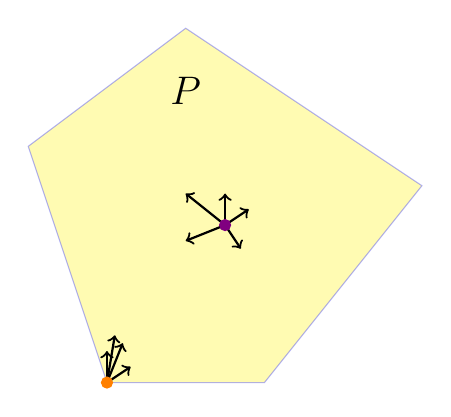
\begin{tikzpicture}
\draw[blue, fill=yellow, opacity=0.3] (0,0) -- (2,1.5) -- (5,-0.5)  -- (3,-3) -- (1,-3) -- cycle;
\draw[->, thick] (2.5,-1) -- (2,-1.2);
\draw[->, thick] (2.5,-1) -- (2.8,-0.8);
\draw[->, thick] (2.5,-1) -- (2.5,-0.6);
\draw[->, thick] (2.5,-1) -- (2,-0.6);
\draw[->, thick] (2.5,-1) -- (2.7,-1.3);
\draw[violet, fill] (2.5,-1) circle [radius=0.7mm];
\draw[->, thick] (1,-3) -- (1.3,-2.8);
\draw[->, thick] (1,-3) -- (1.2,-2.5);
\draw[->, thick] (1,-3) -- (1,-2.6);
\draw[->, thick] (1,-3) -- (1.1,-2.4);
\draw[orange, fill] (1,-3) circle [radius=0.7mm];
\node[] () at (2,0.7) {\Large{\(P\)}};
\end{tikzpicture}
\end{center}
With the concept of feasible direction, we can obtain a sufficient and
necessary condition for optimality, which can be expressed in words as ``moving
along any feasible direction would not reduce the objective function
value''.
\begin{proposition}
\label{prp:optimal-iff-nonneg-feas-dir}
Consider a LP problem of minimization \(\vect{c}^{T}\vect{x}\) over a
polyhedron \(P\).  A point \(\vect{x}^*\in P\) is optimal iff
\(\vect{c}^{T}\vect{d}\ge 0\) for all feasible directions \(\vect{d}\) at
\(\vect{x}^*\).
\end{proposition}
\begin{pf}
``\(\Rightarrow\)'': We prove by contrapositive. Assume
\(\vect{c}^{T}\vect{d}<0\) for some feasible direction \(\vect{d}\) at
\(\vect{x}^*\). Then we can move along that direction to further reduce the
objective function value, since there exists \(\theta>0\) such that
\(\vect{x}^*+\theta\vect{d}\in P\), and we have \(\vect{c}^{T}(\vect{x}^*+\theta\vect{d})
=\vect{c}^{T}\vect{x}+\theta\vect{c}^{T}\vect{d}<\vect{c}^{T}\). Hence
\(\vect{x}^*\) is not optimal.

``\(\Leftarrow\)'': Assume \(\vect{c}^{T}\vect{d}\ge 0\) for all feasible
directions \(\vect{d}\) at \(\vect{x}^*\). Fix any \(\vect{y}\in P\).
Since \(\vect{d}=\vect{y}-\vect{x}^*\) is a feasible direction at
\(\vect{x}^*\) (consider \(\theta=1\)), we have \(\vect{c}^{T}\vect{d}\ge 0\),
which implies \(\vect{c}^{T}\vect{y}\ge\vect{c}^{T}\vect{x}^*\), thus
\(\vect{x}^*\) is optimal.
\end{pf}

While \Cref{prp:optimal-iff-nonneg-feas-dir} provides a sufficient and
necessary condition for optimality, it requires an \emph{infinite} amount of
computations (as there are infinitely many feasible directions in general!).
So we are not satisfied with this condition and will continue our search
\faIcon{search} for a verifiable sufficient condition for optimality.

\item \label{it:feas-dir-bfs} \textbf{Feasible directions at basic feasible
solutions.} Observe from the picture above that there are ``fewer'' feasible
directions at basic feasible solutions (vertices), so if we would like to
``simplify'' the optimality condition in \Cref{prp:optimal-iff-nonneg-feas-dir}
to a condition that is practically verifiable, it appears that we should focus
on optimality condition for basic feasible solutions.

We start by studying the feasible directions at basic feasible solutions. 
\begin{proposition}
\label{prp:feas-dir-bfs}
Let \(P=\{\vect{x}\in\R^n:A\vect{x}=\vect{b}, \vect{x}\ge\vect{0}\}\) be a
standard form polyhedron, where \(A\in\R^{m\times n}\) and \(\vect{b}\in\R^m\),
with rows of \(A\) being linearly independent. Let \(\vect{x}\) be a basic
feasible solution of \(P\) with the corresponding basis matrix
\(B=\begin{bmatrix}\vect{A}_{B(1)}&\cdots&\vect{A}_{B(m)}\end{bmatrix}\). Write
\(\vect{d}=(d_1,\dotsc,d_n)\), \(\vect{d}_{B}:=(d_{B(1)},\dotsc,d_{B(m)})\),
\(\vect{d}_{N}:=(d_{N(1)},\dotsc,d_{N(n-m)})\), and
\(N:=\begin{bmatrix}\vect{A}_{N(1)}&\cdots&\vect{A}_{N(n-m)}\end{bmatrix}\),
where \(N(1),\dotsc,N(n-m)\) are the indices corresponding to the non-basic
variables.

\begin{enumerate}
\item If \(\vect{d}\) is a feasible direction at \(\vect{x}\), then
\(\vect{d}_{B}=-B^{-1}N\vect{d}_{N}\) and \(\vect{d}_{N}\ge
\vect{0}\).
\item If \(\vect{d}_{B}=-B^{-1}N\vect{d}_{N}\), \(\vect{d}_{N}\ge
\vect{0}\), \emph{and \(\vect{x}\) is nondegenerate}, then \(\vect{d}\) is a
feasible direction at \(\vect{x}\).
\end{enumerate}

\end{proposition}
\begin{pf}
\begin{enumerate}
\item Since \(\vect{d}\) is a feasible direction at \(\vect{x}\), we have
\(\vect{x}+\theta\vect{d}\in P\) for some \(\theta>0\). This means that (i)
\(A(\vect{x}+\theta\vect{d})=\vect{b}\) and (ii)
\(\vect{x}+\theta\vect{d}\ge\vect{0}\). From (i), we have \(A\vect{x}+\theta
A\vect{d}=\vect{b}\implies \theta
A\vect{d}=\vect{b}-A\vect{x}\overset{(\vect{x}\in P)}{=}\vect{0} \implies
A\vect{d}=\vect{0}\). By writing \(A\vect{d}=B\vect{d}_{B}+N\vect{d}_{N}\), we
deduce that \(\vect{d}_{B}=-B^{-1}N\vect{d}_{N}\).

Next, note that \(\vect{x}_{N}=\vect{0}\) by \Cref{thm:std-form-basic-sol}.
Hence, from (ii) we have
\(\vect{x}+\theta\vect{d}\ge\vect{0}\overset{\text{(only consider non-basic
ones)}}{\implies} \vect{x}_{N}+\theta\vect{d}_{N}\ge\vect{0}\implies
\vect{d}_{N}\ge\vect{0}\).
\item Assume \(\vect{d}_{B}=-B^{-1}N\vect{d}_{N}\), \(\vect{d}_{N}\ge
\vect{0}\), and \(\vect{x}\) is a nondegenerate basic feasible solution of \(P\).
Then, we have \(A\vect{d}=B\vect{d}_{B}+N\vect{d}_{N}
=-BB^{-1}N\vect{d}_{N}+N\vect{d}_{N}=-N\vect{d}_{N}+N\vect{d}_{N}=\vect{0}\).
Therefore, \(A(\vect{x}+\theta\vect{d})=A\vect{x}+\theta A\vect{d}=\vect{b}\)
for all \(\theta>0\). So it suffices to find a \(\theta>0\) such that
\(\vect{x}+\theta\vect{d}\ge 0\).

For non-basic variables, we always have
\(\vect{x}_{N}+\theta\vect{d}_{N}=\vect{0}+\theta\vect{d}_{N}\ge \vect{0}\),
for every \(\theta>0\). Hence we only need to consider the basic variables.
Since \(\vect{x}\) is a nondegenerate basic feasible solution, we must have
\(x_{B(1)},\dotsc,x_{B(m)}>0\). Therefore, we can choose a sufficiently small
\(\theta>0\) such that \(\vect{x}_{B}+\theta\vect{d}_{B}\ge\vect{0}\).
\begin{note}
More precisely, we can choose
\(\theta=\min_{i=1,\dotsc,m:d_{B(i)}<0}\{-x_{B(i)}/d_{B(i)}\}\)\footnote{This
expression will appear again later in the development of the simplex method.}
if \(d_{B(i)}<0\) for some \(i=1,\dotsc,m\), and can choose any \(\theta>0\) if
\(d_{B(i)}\ge 0\) for all \(i=1,\dotsc,m\).
\end{note}
Thus, with this \(\theta>0\), we have \(\vect{x}+\theta\vect{d}\ge\vect{0}\).
\end{enumerate}
\end{pf}
\item \textbf{Verifiable optimality condition for basic feasible solutions.}
Knowing the properties of feasible directions from \Cref{prp:feas-dir-bfs}, we
can obtain a verifiable optimality condition for basic feasible solutions of
standard form polyhedra.

\begin{proposition}
\label{prp:bfs-optim-nonneg-redu-cost}
Consider a standard form LP problem: minimizing \(\vect{c}^{T}\vect{x}\) over a
standard form polyhedron
\(P=\{\vect{x}\in\R^n:A\vect{x}=\vect{b},\vect{x}\ge\vect{0}\}\).  Let
\(\vect{x}\) be a basic feasible solution. Write \(\vect{c}=(c_1,\dotsc,c_n)\),
\(\vect{c}_{B}:=(c_{B(1)},\dotsc,c_{B(m)})\), and
\(\vect{c}_{N}:=(c_{N(1)},\dotsc,c_{N(n-m)})\). For every \(j=1,\dotsc,n\), let
\(\bar{c}_j:=c_{j}-\vect{c}_{B}^{T}B^{-1}\vect{A}_j\) denote the \defn{reduced
cost} of \(x_j\) (at \(\vect{x}\)). Then:
\begin{enumerate}
\item If \(\bar{c}_j\ge 0\) for all \(j=N(1),\dotsc,N(n-m)\), then
\(\vect{x}\in P\) is optimal.
\item If \(\vect{x}\in P\) is optimal and \emph{nondegenerate}, then
\(\bar{c}_j\ge 0\) for all \(j=N(1),\dotsc,N(n-m)\).
\end{enumerate}
\end{proposition}
\begin{pf}
\begin{enumerate}
\item Assume that \(\bar{c}_j\ge 0\) for all \(j=N(1),\dotsc,N(n-m)\).  Fix any
feasible direction \(\vect{d}\) at \(\vect{x}\). Then, by
\Cref{prp:feas-dir-bfs}, we have \(\vect{d}_{B}=-B^{-1}N\vect{d}_{N}\) and
\(\vect{d}_{N}\ge \vect{0}\). Hence,
\begin{align*}
\vect{c}^{T}\vect{d}&=\vect{c}_{B}^{T}\vc{\vect{d}_{B}}+\vect{c}_{N}^{T}\vect{d}_{N}
=\vc{-}\vect{c}_{B}^{T}\vc{B^{-1}N\vect{d}_{N}}+\vect{c}_{N}^{T}\vect{d}_{N} \\
&=(\vect{c}_{N}^{T}-\vect{c}_{B}^{T}B^{-1}N)\vect{d}_{N}
=\sum_{i=1}^{n-m}\left(c_{N(i)}-\vect{c}_{B}^{T}B^{-1}\vect{A}_{N(i)}\right)d_{N(i)}
=\sum_{i=1}^{n-m}\underbrace{\bar{c}_{N(i)}}_{\ge 0}\underbrace{d_{N(i)}}_{\ge 0}
\ge 0.
\end{align*}
Thus, by \Cref{prp:optimal-iff-nonneg-feas-dir} we conclude that \(\vect{x}\)
is optimal.  \item Assume to the contrary that \(\vect{x}\in P\) is optimal and
nondegenerate, but \(\bar{c}_j<0\) for some \(j=N(1),\dotsc,N(n-m)\). Then, by
setting \(\vect{d}_j=1\), \(\vect{d}_{j'}=0\) all non-basic indices \(j'\ne
j\), and \(\vect{d}_{B}=-B^{-1}N\vect{d}_{N}\) (this will appear again in
\labelcref{it:reduced-cost}), we know by \Cref{prp:feas-dir-bfs} that
\(\vect{d}\) is a feasible direction at \(\vect{x}\), so \(\vect{x}+\theta \vect{d}\in P\)
for some \(\theta>0\).

But then by construction we would have
\(\vect{c}^{T}\vect{d}\overset{\text{(see above)}}{=}
\sum_{i=1}^{n-m}\bar{c}_{N(i)}d_{N(i)}=\bar{c}_j<0\), implying that
\(\vect{c}^{T}(\vect{x}+\theta d)<\vect{c}^{T}\vect{d}\), contradicting to the
optimality of \(\vect{x}\).
\end{enumerate}
\end{pf}

\begin{remark}
\item This optimality condition is \emph{verifiable} as it only involves checking
\(n-m\) signs \cmark.
\item Due to \Cref{prp:bfs-optim-nonneg-redu-cost}, a basis matrix \(B\) is said to be
\defn{optimal} if (i) \(\vect{x}_{B}=B^{-1}\vect{b}\ge\vect{0}\)
\emph{(feasibility)} and (ii) \(\bar{c}_j\ge 0\) for all \(j=N(1),\dotsc,N(n-m)\)
\emph{(optimality)}. If we have obtained a basic feasible solution with \underline{optimal}
basis matrix, then such basic feasible solution must be \underline{optimal}.
Also, every nondegenerate \underline{optimal} basic feasible solution must
admit an \underline{optimal} basis matrix.
\end{remark}

\item \label{it:reduced-cost} \textbf{More about reduced cost.} To interpret
reduced cost, in the equation
\(\vect{c}^{T}\vect{d}=\sum_{i=1}^{n-m}\bar{c}_{N(i)}\vect{d}_{N(i)}\) from the
proof above, we can set \(\vect{d}_{j}=1\), \(\vect{d}_{j'}=0\) for all
non-basic indices \(j'\ne j\), and \(\vect{d}_{B}=-B^{-1}N\vect{d}_{N}\). This
gives \(\vect{c}^{T}\vect{d}=\bar{c}_j\), which suggests that the reduced cost
\(\bar{c}_j\) of \(x_j\) refers to the rate of change \(\vect{c}^{T}\vect{d}\)
of objective function value (or \underline{cost}) when moving along such
direction \(\vect{d}\); this is the change in cost per unit increase in \(x_j\)
(namely \(c_j\)), \underline{reduced} by the amount
\(\vect{c}_{B}^{T}B^{-1}\vect{A}_j\) (serving as an adjustment for the changes
in basic variables from moving along such direction).

With this interpretation, it should be intuitive that the reduced cost of any
basic variable \(x_j\) is always zero, as the adjustment would intuitively
reduce the whole rate of change of cost from the increase in basic variable. It
can also be mathematically proved as follows:

\begin{pf}
Since \(x_j\) is a basic variable, we know \(j=B(k)\) for some
\(k=1,\dotsc,m\). Hence, we have \(B^{-1}\vect{A}_j
=B^{-1}\vect{A}_{B(k)}
=\vect{e}_k\)
(note that \(I_m=B^{-1}B=B^{-1}\begin{bmatrix}\vect{A}_{B(1)}&\cdots&\vect{A}_{B(m)}\end{bmatrix}
=\begin{bmatrix}B^{-1}\vect{A}_{B(1)}&\cdots&B^{-1}\vect{A}_{B(m)}\end{bmatrix}
\)). Therefore, the reduced cost is
\[
\bar{c}_{j}=c_j-\vect{c}_{B}^{T}B^{-1}\vect{A}_{j}
=c_j-\vect{c}_{B}^{T}\vect{e}_k
=c_j-c_{B(k)}
=c_j-c_j=0.
\]
\end{pf}

Because of this, we can rewrite the optimality condition from
\Cref{prp:bfs-optim-nonneg-redu-cost} in the \emph{row} vector form:
\((\bar{c}_{1},\dotsc,\bar{c}_{n})^{T}=:\bar{\vect{c}}^{T}\ge\vect{0}\), where
we have \(\bar{\vect{c}}^{T}=\vect{c}^{T}-\vect{c}_{B}^{T}B^{-1}A\) (here
\(\vect{0}\) denotes zero \emph{row} vector). In words, this means a basic
feasible solution is optimal if the reduced costs (of all variables) are
nonnegative.
\end{enumerate}
\subsection{Development and Implementation of the Simplex Method}
\label{subsect:simplex-dev-implement}
\begin{enumerate}
\item \textbf{Intuition for the simplex method.}
Before looking into the details of the simplex method, we
first study the main idea behind the simplex method.  Consider
a standard form LP problem:
\begin{align*}
\text{min}\quad&\vect{c}^{T}\vect{x} \\
\text{s.t.}\quad&A\vect{x}=\vect{b} \\
&\vect{x}\ge \vect{0}
\end{align*}
where \(A\in\R^{m\times n}\) (with rows being linearly independent) and
\(\vect{b}\in\R^m\).
Let us collect some previous results about the standard form LP problem below:
\begin{enumerate}[label={(\arabic*)}]
\item (\Cref{thm:vertex-optimal}) If the optimal value is finite, then it must be achieved at one of the
basic feasible solutions.
\item (\labelcref{it:std-form-bfs-procedure}) A standard form polyhedron only has finitely many basic feasible solutions.
\item (\labelcref{it:reduced-cost}) A basic feasible solution is optimal if the
reduced costs are nonnegative.
\end{enumerate}
Based on the results (1) and (2) alone, we can already obtain a straightforward
method (``high school approach'') for solving standard form LP problems as
follows: Assuming that the optimal value is finite, we can compute the
objective function value at each of the finitely many basic feasible solutions,
and the smallest value is the optimal value, with the corresponding basic
feasible solution(s) being the optimal solution(s).

However, this method has some disadvantages \faIcon[regular]{thumbs-down}:
\begin{itemize}
\item \emph{(assumption on the finiteness of optimal value)} The optimal value
is required to be finite, but we may not know whether this is the case before
solving the LP problem.
\item \emph{(computational cost)} When the values of \(m\) and \(n\) are large,
there would be a very large number of basic feasible solutions to be
considered, leading to a high computational cost.
\end{itemize}
The \emph{simplex method} to be developed here does not have these
disadvantages (though it is less straightforward). Apart from the results
(1)-(2), it also utilizes (3), which provides us a sufficient condition for
optimality. The key \faIcon{key} idea of the simplex method is to \emph{move
between basic feasible solutions until the reduced costs are all nonnegative},
i.e., going through the finitely many basic feasible solutions and checking the
optimality of each of them in the process (whether the reduced costs are all
nonnegative or not).

\item\label{it:simplex-method-dir-mag} \textbf{Implementation details for the simplex method.}
While the intuitive idea of the simplex method is given above, it is not enough
for the actual implementation; we also need to specify how such ``movements
between basic feasible solutions'' should take place. To be more precise, we
need to figure out a way to determine both the \emph{direction} and
\emph{magnitude} of the next movement in the algorithm, starting from a certain
basic feasible solution \(\vect{x}\) at which the reduced costs are not yet all
nonnegative, say \(\bar{c}_{j}<0\) for some non-basic index \(j\). Unless
otherwise specified, we shall assume throughout that every basic feasible
solution is \emph{nondegenerate}.

For the \emph{direction}, we should naturally move along a feasible direction where the
objective function value decreases (as we are solving a minimization problem).
Recall from \labelcref{it:reduced-cost} that we have
\(\vect{c}^{T}\vect{d}=\bar{c}_j\) if we set \(d_j=1\) and \(d_{j'}=0\) for all
non-basic indices \(j'\ne j\). Since we have \(\bar{c}_j<0\) here, moving along such
direction would lead to a change of \(\vect{c}^{T}\vect{d}<0\) in the objective
function value (a decrease), which is what we want. Hence, we will choose the
direction \(\vect{d}\) as follows:
\begin{itemize}
\item \emph{(non-basic variables)} \(\boxed{d_{j}=1}\) and \(\boxed{d_{j'}=0}\) for all
non-basic indices \(j'\ne j\).
\item \emph{(basic variables)} \(\boxed{\vect{d}_{B}}=-B^{-1}N\vect{d}_{N}
\overset{\text{(\(j=N(i)\) for some \(i\))}}{=}
-B^{-1}N\vect{e}_i
=-B^{-1}\vect{A}_{N(i)}
\boxed{=-B^{-1}\vect{A}_j}\)
\end{itemize}
\begin{note}
Under nondegeneracy, this direction \(\vect{d}\) must be a feasible direction
by \Cref{prp:feas-dir-bfs}.
\end{note}

For the \emph{magnitude}, we are referring to the value of \(\theta>0\) in
\(\vect{y}=\vect{x}+\theta\vect{d}\) where \(\vect{y}\) is the destination of
the movement. Since we have \(\vect{c}^{T}\vect{d}<0\) from above, naturally we
would like to set \(\theta\) as large as possible so that the decrease in the
objective function value is maximized. However, it may be possible that
\(\vect{y}=\vect{x}+\theta\vect{d}\notin P\) if the \(\theta\) chosen is too
large.

Inspired by the proof of \Cref{prp:feas-dir-bfs}, we set the \(\theta\) as:
\[
\boxed{\theta^{*}=\min_{i=1,\dotsc,m:d_{B(i)}<0}\left\{-\frac{x_{B(i)}}{d_{B(i)}}\right\}}
\]
if \(d_{B(i)}<0\) for some \(i=1,\dotsc,m\), which is the largest possible
\(\theta\) to ensure that the basic variables are still nonnegative
(thus remaining feasible) in this case.

If we have \(d_{B(i)}\ge 0\) for all \(i=1,\dotsc,m\), it means that
\(\vect{x}+\theta\vect{d}\) remains feasible for all \(\theta>0\), so we can
set \(\theta\) to be arbitrarily large. But in such case, it implies that the
objective function value can be arbitrarily negative, and hence the objective
function is not bounded below in the feasible region, making the optimal value
\(-\infty\).
\item \textbf{A change-of-basis point of view of the simplex method.} Following
the steps put forward in \labelcref{it:simplex-method-dir-mag}, assuming
\(d_{B(i)}<0\) for some \(i=1,\dotsc,m\), we will move from the starting basic
feasible solution \(\vect{x}\) to another point
\(\vect{x}^{*}=\vect{x}+\theta^{*}\vect{d}\in P\) (which is indeed another basic
feasible solution of \(P\), to be shown in \Cref{prp:change-of-basis-simplex}).

Let \(\ell\) be a minimizing index for the formula of \(\theta^{*}\), i.e.,
\(-x_{B(\ell)}/d_{B(\ell)} =\theta^{*}\), which implies that
\(x_{B(\ell)}^{*}=x_{B(\ell)}+\theta^{*}d_{B(\ell)}=0\), meaning that the
variable with index \(B(\ell)\) in \(\vect{x}^*\) becomes zero.  On the other
hand, since \(x_j=0\) and \(d_j=1\), we have
\(x_j^{*}=0+\theta^{*}(1)=\theta^{*}>0\). Therefore, after an iteration in the
simplex method, (i) a variable with basic index originally
(\(x_{B(\ell)}^{*}\)) becomes zero and (ii) a variable with nonbasic index
originally (\(x_j^{*}\)) becomes positive.

Naturally, this suggests us to replace the column \(\vect{A}_{B(\ell)}\) in the
original basis by the column \(\vect{A}_j\), forming a new matrix
\begin{align*}
\bar{B}&=\begin{bmatrix}
\vect{A}_{B(1)}&\vect{A}_{B(\ell -1)}&\vect{A}_j&\vect{A}_{B(\ell+1)}&\cdots&\vect{A}_{B(m)}
\end{bmatrix} \\
&=\begin{bmatrix}
\vect{A}_{\bar{B}(1)}&\vect{A}_{\bar{B}(\ell -1)}&\vect{A}_{\bar{B}(\ell)}&\vect{A}_{\bar{B}(\ell+1)}
&\cdots&\vect{A}_{\bar{B}(m)}
\end{bmatrix},
\end{align*}
where \(\bar{B}(i)=B(i)\) for all \(i\ne\ell\) and \(\bar{B}(\ell)=j\).
We say that the column
\(\vect{A}_{B(\ell)}\) \defn{exits the basis} and the column \(\vect{A}_j\)
\defn{enters the basis} in this case. Let us justify that such matrix
\(\bar{B}\) is indeed a basis matrix and we can view \(\vect{x}^*\) as a basic
feasible solution associated with the basis matrix \(\bar{B}\) below.

\begin{proposition}
\label{prp:change-of-basis-simplex}
\hfill
\begin{enumerate}
\item The columns
\(\vect{A}_{B(1)},\dotsc,\vect{A}_{B(\ell-1)},\vect{A}_j,\vect{A}_{B(\ell+1)},\dotsc,\vect{A}_{B(m)}\)
are linearly independent (hence \(\bar{B}\) is a basis matrix).
\item \(\vect{x}^*=\vect{x}+\theta^{*}\vect{d}\) is a basic feasible solution
of \(P\) associated with the basis matrix \(\bar{B}\).
\end{enumerate}
\end{proposition}
\begin{pf}
\begin{enumerate}
\item By a result from linear algebra,
\(\vect{A}_{B(1)},\dotsc,\vect{A}_{B(\ell-1)},\vect{A}_j,\vect{A}_{B(\ell+1)},\dotsc,\vect{A}_{B(m)}\)
are linearly independent iff \(B^{-1}\vect{A}_{B(1)},\dotsc,B^{-1}\vect{A}_{B(\ell-1)},
B^{-1}\vect{A}_j,B^{-1}\vect{A}_{B(\ell+1)},\dotsc,B^{-1}\vect{A}_{B(m)}\) are
linearly independent. So we will prove the latter.

Since \(\begin{bmatrix}B^{-1}\vect{A}_{B(1)}&\cdots&B^{-1}\vect{A}_{B(m)}\end{bmatrix}
=B^{-1}B=I_m\), we know \(B^{-1}\vect{A}_{B(i)}=\vect{e}_i\) for all \(i\ne\ell\), which particularly means
that their \(\ell\)th entries are all zero.

On the other hand, we have \(B^{-1}\vect{A}_j=-\vect{d}_{B}\), whose \(\ell\)th
entry is \(-\vect{d}_{B(\ell)}>0\) (as \(\vect{d}_{B(\ell)}<0\) by the
definition of \(\ell\)). This means that \(B^{-1}\vect{A}_j\) is not a linear
combination of \(B^{-1}\vect{A}_{B(i)},\quad i\ne\ell\) (which are linearly
independent among themselves). The desired result then follows by the extension
approach from linear algebra.
\item By construction of \(\theta^{*}\) and \(\vect{d}\), we have
\(A\vect{x}^*=\vect{b}\) and \(\vect{x}^{*}\ge\vect{0}\), so \(\vect{x}^*\) is
feasible. Also, for all \(i\notin\{\bar{B}(1),\dotsc,\bar{B}(m)\}\), we have
either \(i=B(\ell)\) or \(i=j'\) where \(j'\) is an original non-basic index
different from \(j\). In the former case, \(x_i^{*}=x_{B(\ell)}=0\) as
discussed above. In the latter case, \(x_i^{*}=x_{j'}^{*}=x_{j'}+\theta
d_{j'}=x_{j'}+0\overset{\text{(\(x_{j'}\) non-basic)}}{=}0\). So \(x_i^*=0\)
for all \(i\notin\{\bar{B}(1),\dotsc,\bar{B}(m)\}\), and
\(\sum_{i=1}^{m}\vect{A}_{\bar{B}(i)}x^*_{\bar{B}(i)}=A\vect{x}^{*}=\vect{b}\).

Together with the linear independence
\(\vect{A}_{\bar{B}(1)},\dotsc,\vect{A}_{\bar{B}(m)}\) (shown above), we
conclude that \(\vect{x}^*\) is a basic feasible solution of \(P\) by
\Cref{thm:std-form-basic-sol}, associated with the basis matrix \(\bar{B}\).
\end{enumerate}
\end{pf}
\item \label{it:simplex-method-algo} \textbf{Summary of the simplex method.}
Based on the previous results, we can summarize the procedures carried out in
the \defn{simplex method} as follows.
\begin{enumerate}[label={(\arabic*)}]
\item Start with a basic feasible solution \(\vect{x}\) with basis matrix \(B=\begin{bmatrix}
\vect{A}_{B(1)}&\cdots&\vect{A}_{B(m)}\end{bmatrix}\), which is given by
\(\vect{x}_{B}=B^{-1}\vect{b}\) and \(\vect{x}_N=\vect{0}\) (see
\labelcref{it:std-form-bfs-procedure}).
\item Compute the reduced costs
\(\bar{c}_j=c_j-\vect{c}_{B}^{T}B^{-1}\vect{A}_j\) for all non-basic indices
\(j\).
\begin{enumerate}
\item If \(\bar{c}_j\ge 0\) for all non-basic indices \(j\), then the current
basic feasible solution \(\vect{x}\) is optimal, and the algorithm terminates
\faIcon[regular]{pause-circle}.
\item Otherwise, fix a non-basic index \mgc{\(j\)} with \(\bar{c}_{\mgc{j}}<0\).
\end{enumerate}
\item Compute \(\vect{u}=B^{-1}\vect{A}_{\mgc{j}}\) (which equals
\(-\vect{d}_{B}\)).
\begin{enumerate}
\item If no entry of \(\vect{u}\) is positive, then the optimal value is
\(-\infty\), and the algorithm terminates \faIcon[regular]{pause-circle}.
\item If some entries of \(\vect{u}\) are positive, set
\[
\theta^{*}=\min_{i=1,\dotsc,m:u_i>0}\left\{\frac{x_{B(i)}}{u_i}\right\}.
\]
\end{enumerate}
\item Let \(\ell\) be a minimizing index, i.e.,
\(x_{B(\ell)}/u_{\ell}=\theta^{*}\). Form a new basis matrix \(\bar{B}\) by
replacing the column \(\vect{A}_{B(\ell)}\) by \(\vect{A}_{\mgc{j}}\). For the new
basic feasible solution \(\vect{x}^*\), the basic variables are given by
\(x_{B(i)}^{*}=x_{B(i)}-\theta^{*}u_i\) for all \(i\ne\ell\) and
\(x_{\mgc{j}}^{*}=\theta^{*}\) (and the non-basic variables are all zero).
\item Repeat (1)-(4) with the starting basic feasible solution updated to the
new one obtained in the previous iteration, until the algorithm terminates
\faIcon[regular]{pause-circle}.
\end{enumerate}
\begin{remark}
\item We do not need to explicitly compute the movement direction \(\vect{d}\) in the
process.
\item It can be shown that, as long as the feasible region is nonempty and every
basic feasible solution is nondegenerate, the algorithm above must terminate
after a finite number of iterations.
\end{remark}
\item \label{it:simplex-update-binv-eros} \textbf{Updating \(B^{-1}\) through
elementary row operations.} In the simplex method depicted in
\labelcref{it:simplex-method-algo}, one major disadvantage is that it requires
the computation of \(B^{-1}\) in each iteration, which is computationally more
costly than the computations of vector inner products \(\vect{a}^{T}\vect{b}\),
and matrix-vector products \(A\vect{b}\). In view of this deficiency, the
\emph{revised} simplex method is developed to avoid excessive computations of
matrix inverse in the algorithm. The key \faIcon{key} idea is to just compute
\(B^{-1}\) once at the initialization, and only \emph{update} \(B^{-1}\) in a
``smarter'' way, that is less costly than recomputing the matrix inverse, in
the subsequent iterations.

Such update of \(B^{-1}\) is developed based on the observation that, the
change in the basis matrix after an iteration is \(B\to\bar{B}\), in which only
\emph{one} column changes (\(\vect{A}_{B(\ell)}\to \vect{A}_{\bar{B}(\ell)}=\vect{A}_j\)).
As the basis matrix only undergoes a somewhat ``small'' change, it is natural
to expect that the corresponding matrix inverse won't change much also. Indeed,
we can change \(B^{-1}\to\bar{B}^{-1}\) via performing \emph{elementary row
operations} (EROs) only.

From linear algebra, we know that performing EROs corresponds to
left-multiplying elementary matrices. So what we want to do now is to find out
a sequence of elementary matrices \(E_1,\dotsc,E_r\) such that \(E_r\dotsb
E_1B^{-1}=\bar{B}^{-1}\) which can be rewritten as \(E_r\dotsb
E_1B^{-1}\bar{B}=\bar{B}^{-1}\bar{B}=I_m\). This means that it suffices to find
a sequence of EROs that turn \(B^{-1}\bar{B}\) to \(I_m\), which can be
obtained as follows.

Since \(\begin{bmatrix}B^{-1}\vect{A}_{B(1)}&\cdots&B^{-1}\vect{A}_{B(m)}\end{bmatrix}
=B^{-1}B=I_m\), we know \(B^{-1}\vect{A}_{B(\ell)}=\vect{e}_i\) for all
\(i\ne\ell\) (you should have seen this in the proof of
\Cref{prp:change-of-basis-simplex} already). Thus, we can write
\begin{align*}
B^{-1}\bar{B}&=\begin{bmatrix}\vect{e}_1&\cdots&\vect{e}_{\ell-1}&\vect{u}&
\vect{e}_{\ell+1}&\cdots&\vect{e}_m\end{bmatrix} \\
&=\begin{bmatrix}1&\cdots&0&u_1&0&\cdots&0 \\
\vdots&\vdots&\vdots&\vdots&\vdots&\vdots&\vdots \\
0&\cdots&1&u_{\ell-1}&0&\cdots&0 \\
0&\cdots&0&u_{\ell}&0&\cdots&0 \\
0&\cdots&0&u_{\ell+1}&1&\cdots&0 \\
\vdots&\vdots&\vdots&\vdots&\vdots&\vdots&\vdots \\
0&\cdots&0&u_{m}&1&\cdots&1
\end{bmatrix}
\end{align*}
\begin{note}
We have \(\vect{u}=-\vect{d}_{B}=B^{-1}\vect{A}_j\).
\end{note}
From this expression, we can observe that the following sequence of EROs can
turn \(B^{-1}\bar{B}\) to \(I_m\):
\begin{enumerate}[label={(\arabic*)}]
\item \emph{(changing \(u_{\ell}\to 1\))} First perform the ERO
\((1/u_{\ell})\vect{r}_{\ell}\to\vect{r}_{\ell}\).
\begin{note}
We have \(u_{\ell}>0\) by the definition of \(\ell\).
\end{note}
\item \emph{(zeroizing the \(i\)th entry of the column \(\vect{u}\) for all \(i\ne\ell\))}
For all \(i\ne\ell\), perform the ERO
\(-u_i\vect{r}_{\ell}+\vect{r}_{i}\to\vect{r}_{i}\) (i.e., adding
\(-u_i\) times the \(\ell\)th row to the \(i\)th row).
\end{enumerate}
In short, we are adding each of the rows a multiple of the \(\ell\)th row to
make the column corresponding to \(\vect{u}\) equal the vector \(\vect{e}_{\ell}\).

\item\label{it:revised-simplex-algo} \textbf{Revised simplex method.} Building upon the idea in
\labelcref{it:simplex-update-binv-eros}, the \defn{revised simplex method} is
as follows.
\begin{enumerate}[label={(\arabic*)}]
\item Start with a basic feasible solution \(\vect{x}\) with basis matrix \(B=\begin{bmatrix}
\vect{A}_{B(1)}&\cdots&\vect{A}_{B(m)}\end{bmatrix}\), which is given by
\(\vect{x}_{B}=B^{-1}\vect{b}\) and \(\vect{x}_N=\vect{0}\) (see
\labelcref{it:std-form-bfs-procedure}). \vc{At initialization, compute the inverse \(B^{-1}\).}
\item Compute the reduced costs
\(\bar{c}_j=c_j-\vect{c}_{B}^{T}B^{-1}\vect{A}_j\) for all non-basic indices
\(j\).
\begin{enumerate}
\item If \(\bar{c}_j\ge 0\) for all non-basic indices \(j\), then the current
basic feasible solution \(\vect{x}\) is optimal, and the algorithm terminates
\faIcon[regular]{pause-circle}.
\item Otherwise, fix a non-basic index \mgc{\(j\)} with \(\bar{c}_{\mgc{j}}<0\).
\end{enumerate}
\item Compute \(\vect{u}=B^{-1}\vect{A}_{\mgc{j}}\) (which equals
\(-\vect{d}_{B}\)). \begin{note}
The reason why we use the vector \(\vect{u}\) instead of \(\vect{d}_{B}\) here will become transparent later.
\end{note}
\begin{enumerate}
\item If no entry of \(\vect{u}\) is positive, then the optimal value is
\(-\infty\), and the algorithm terminates \faIcon[regular]{pause-circle}.
\item If some entries of \(\vect{u}\) are positive, set
\[
\theta^{*}=\min_{i=1,\dotsc,m:u_i>0}\left\{\frac{x_{B(i)}}{u_i}\right\}.
\]
\end{enumerate}
\item Let \(\ell\) be a minimizing index, i.e.,
\(x_{B(\ell)}/u_{\ell}=\theta^{*}\). Form a new basis matrix \(\bar{B}\) by
replacing the column \(\vect{A}_{B(\ell)}\) by \(\vect{A}_{\mgc{j}}\). For the new
basic feasible solution \(\vect{x}^*\), the basic variables are given by
\(x_{B(i)}^{*}=x_{B(i)}-\theta^{*}u_i\) for all \(i\ne\ell\) and
\(x_{\mgc{j}}^{*}=\theta^{*}\) (and the non-basic variables are all zero).

\item \vc{Form an augmented matrix
\(\begin{bmatrix}B^{-1}|\vect{u}\end{bmatrix}\in\R^{m\times (m+1)}\).
Add each of its rows a multiple of the \(\ell\)th row to make the last
column equal to \(\vect{e}_{\ell}\). After that, the matrix on the left-hand
side would become the inverse of the new basis matrix \(\bar{B}^{-1}\).
}
\item Repeat (1)-(5) with the starting basic feasible solution \vc{and the
inverse of the basis matrix} updated to the new ones obtained in the previous
iteration, until the algorithm terminates \faIcon[regular]{pause-circle}.
\end{enumerate}
\item \textbf{Tableau representation of the simplex method.} While the
procedure of the revised simplex method in \labelcref{it:revised-simplex-algo}
can be implemented in computer program \faIcon{code} to solve standard form LP
problems efficiently, it is still a bit cumbersome to be carried out \emph{by
hand} \faIcon{pen}, due to the numerous quantities to be tracked and computed.
Here, we will introduce a method, known as \emph{tableau representation}
\faIcon{table}, that allows us to carry out the simplex method by hand in a
much more convenient way.

In the simplex method, we have been maintaining and updating the matrix
\(B^{-1}\) in each iteration. In the tableau representation, instead of dealing
with \(B^{-1}\), we maintain the matrix (or \defn{tableau})
\(B^{-1}[\vect{b}|A]
=\begin{bmatrix}B^{-1}\vect{b}&B^{-1}\vect{A}_1&\cdots&B^{-1}\vect{A}_n\end{bmatrix}\).
Conventionally, the column \(B^{-1}\vect{b}\) is called the \defn{zeroth
column} instead of the first column, and the column \(B^{-1}\vect{A}_i\) is
called the \(i\)th column (perhaps following the logic of zero-based indexing
in coding \faIcon{code}?).

\begin{remark}
\item \emph{(Rationale for maintaining the matrix \(B^{-1}[\vect{b}|A]\))}
Note that left-multiplying \(B^{-1}\) on both sides of the equality constraints
\(\vect{b}=A\vect{x}\) gives \(B^{-1}\vect{b}=B^{-1}\vect{A}\vect{x}\). So the matrix
\(B^{-1}[\vect{b}|A]\) actually collects the coefficients of
\(B^{-1}\vect{b}=B^{-1}\vect{A}\vect{x}\), which contain useful information for
carrying out the simplex method.
\item \emph{(Zeroth column contains basic variables)} Recall from
\labelcref{it:std-form-bfs-procedure} that
\(A\vect{x}_{B}=B\vect{x}_{B}=\vect{b}\), so the vector of basic variables
\(\vect{x}_B\) is given by \(B^{-1}\vect{b}\), which is precisely the zeroth
column here.
\end{remark}
\item \textbf{Performing some steps in the revised simplex method through the
tableau.}
After studying what the tableau is, we now consider how we should utilize it to
perform the steps in the revised simplex method as suggested in
\labelcref{it:revised-simplex-algo}. For now, we focus on the steps (3)-(5); we
will consider the rest in \labelcref{it:tableau-implement}.

\begin{itemize}
\item[(3)] Suppose that we are in the case where some entries of
\(\vect{u}=B^{-1}\vect{A}_j\) (the \(j\)th column of the tableau; also known as
the \defn{pivot column}) are positive.  (Otherwise, the algorithm would have
been terminated already.) Then we consider the tableau:
\begin{center}
\begin{tikzpicture}
\node[] () at (0,0) {
\(
\begin{bmatrix}
x_{B(1)}&\cdots&\mgc{u_1}&\cdots \\
x_{B(2)}&\cdots&\mgc{u_2}&\cdots \\
\vdots&\ddots&\mgc{\vdots}&\vdots \\
x_{B(m)}&\cdots&\mgc{u_m}&\cdots \\
\end{bmatrix}
\)
};
\node[] () at (-1.3,1.5) {\small{(0th col.)}};
\node[] () at (0.7,1.5) {\mgc{\small{(pivot col.)}}};
\end{tikzpicture}
\end{center}
For every row \(i=1,\dotsc,m\), if \(u_i>0\), we compute the ratio
\(x_{B(i)}/u_{i}\). The index with the smallest ratio obtained is then the
minimizing index \(\ell\), and such ratio \(x_{B(\ell)}/u_{\ell}\) equals
\(\theta^*\). That \(\ell\)th row is also known as the \defn{pivot row}.  The
element that belongs to both the pivot column and the pivot row is called the
\defn{pivot element}, which is \(u_{\ell}\) here.
\item[(4-5)] Here we would like to update the tableau \(B^{-1}[\vect{b}|A]\) to
\(\bar{B}^{-1}[\vect{b}|A]\), where \(\bar{B}\) being the new basis matrix as
specified in step (4). This can be done by performing EROs on the tableau in
the way suggested by the step (5) in \labelcref{it:revised-simplex-algo}, i.e.,
adding each of its rows a multiple of the \emph{pivot row} to make all entries of the
\emph{pivot column} zero, except the \emph{pivot element}, which is set to one.

We can also observe that, after performing such EROs, the zeroth column does
contain the basic variables for the \emph{new} basic feasible solution \(\vect{x}^{*}\)
(compare the EROs with the formulas in step (4)). Thus, performing these EROs
allows us to do two things at once.
\begin{center}
\begin{tikzpicture}
\node[] () at (0,0) {
\(
\begin{bmatrix}
x_{B(1)}&\cdots&\mgc{u_1}&\cdots \\
x_{B(2)}&\cdots&\mgc{u_2}&\cdots \\
\vdots&\ddots&\mgc{\vdots}&\vdots \\
\mgc{x_{B(\ell)}}&\mgc{\cdots}&\mgc{\boxed{u_\ell}}&\mgc{\cdots} \\
\vdots&\ddots&\mgc{\vdots}&\vdots \\
x_{B(m)}&\cdots&\mgc{u_m}&\cdots \\
\end{bmatrix}
\)
};
\node[] () at (-1.3,2) {\small{(0th col.)}};
\node[] () at (0.7,2) {\mgc{\small{(pivot col.)}}};
\node[] () at (-3,-0.2) {\mgc{\small{(pivot row)}}};
\draw[-Latex] (3.5,0.2) -- (0.8,1.3);
\draw[-Latex] (3.5,0.2) -- (0.8,0.9);
\draw[-Latex] (3.5,0.2) -- (0.8,0.3);
\draw[-Latex] (3.5,0.2) -- (0.8,-0.8);
\draw[-Latex] (3.5,0.2) -- (0.8,-1.2);
\node[] () at (4.8,0.2) {make them zero};
\draw[-Latex, blue] (3.5,-1) -- (0.8,-0.2);
\node[blue] () at (4.5,-1) {make it one};
\end{tikzpicture}
\end{center}
\end{itemize}
\item \label{it:tableau-implement} \textbf{Implementing the simplex method
iterations through the tableau.} To implement the full simplex method, it is
convenient to add one extra row (known as the \defn{zeroth row}) at the top of
the tableau, which contains the \emph{negative} objective function value
\(-\vect{c}^{T}\vect{x}=-\vect{c}_{B}^{T}\vect{x}_{B}=-\vect{c}_{B}^{T}B^{-1}\vect{b}\) and the row
vector of reduced costs
\(\bar{\vect{c}}^{T}=\vect{c}^{T}-\vect{c}_{B}^{T}B^{-1}A\):
\begin{center}
\begin{tabular}{cc}
\toprule
\(-\vect{c}_{B}^{T}B^{-1}\vect{b}\)&\(\vect{c}^{T}-\vect{c}_{B}^{T}B^{-1}A\) \\
\midrule
\(B^{-1}\vect{b}\)&\(B^{-1}A\) \\
\bottomrule
\end{tabular}
\end{center}
It can be expressed more explicitly as:
\begin{center}
\begin{tabular}{cccc}
\toprule
\(-\vect{c}_{B}^{T}\vect{x}_{B}\)&\(\bar{c}_1\)&\(\cdots\)&\(\bar{c}_{n}\) \\
\midrule
\(x_{B(1)}\)&\(\vert\)&&\(\vert\) \\
\(\vdots\)&\(B^{-1}\vect{A}_1\)&\(\cdots\)&\(B^{-1}\vect{A}_n\) \\
\(x_{B(m)}\)&\(\vert\)&&\(\vert\) \\
\bottomrule
\end{tabular}
\end{center}
With the zeroth row added, we can perform the step (2) conveniently: just find
out a column with negative reduced cost by inspection (assuming some reduced
costs are negative), which corresponds to the non-basic index \(j\). For the
step (1), the initial choice of the basic feasible solution \(\vect{x}\) is an
\emph{input} to this tableau method, and can be obtained as in
\labelcref{it:std-form-bfs-procedure}.

It now remains to handle the update of the zeroth row in each iteration. After
having the new basis matrix \(\bar{B}\) from the previous iteration, we need to
update the reduced costs and also the negative objective function value. As it
turns out, the ``rule'' for updating the zeroth row works exactly the same as
that for the other rows, namely adding a multiple of the pivot row to the
zeroth row to make the entry at the pivot column (the ``\(\bar{c}_j\)''
originally) zero. This ``rule'' does not directly follow from the previous
discussions on revised simplex method, and we will justify it in the following.

\begin{pf}
At the beginning of iteration, the zeroth row takes the form
\([0|\vect{c}^{T}]-\vect{g}^{T}[\vect{b}|A]\) where
\(\vect{g}^{T}=\vect{c}_{B}^{T}B^{-1}\). Let column \(j\) and row \(\ell\) be
the pivot column and the pivot row respectively. Since the pivot row takes the
form \(\vect{h}^{T}[\vect{b}|A]\) (where \(\vect{h}^{T}\) is the \(\ell\)th row
of \(B^{-1}\)), adding a multiple of the pivot row to the zeroth row converts
it to a row of the form \([0|\vect{c}^{T}]-\vect{p}^{T}[\vect{b}|A]\) for some
vector \(\vect{p}\).

Since the ERO we perform makes the pivot column entry of the zeroth row \(0\),
we have \(c_{\bar{B}(\ell)}-\vect{p}^{T}\vect{A}_{\bar{B}(\ell)}=c_j-\vect{p}^{T}\vect{A}_j=0\)
(note that \(j=\bar{B}(\ell)\)). Now, consider the \(\bar{B}(i)\)th column with
\(i\ne\ell\), which corresponds to a original basic variable that stays in the
new basis, so we know its zeroth row entry is \(0\) before the ERO. Also, for
all \(i\ne\ell\), we have \(B^{-1}\vect{A}_{B(i)}=\vect{e}_i\) (as it is the
\(i\)th column of the identity matrix \(I_m=B^{-1}B\)), meaning that the pivot
row (\(\ell\ne i\)th row) entry of the \(i\)th column is also \(0\). Hence,
after such ERO we know the zeroth row entry of the \(\bar{B}(i)\)th column is
still \(0\). Therefore, the vector \(\vect{p}\) satisfies
\(c_{\bar{B}(i)}-\vect{p}^{T}\vect{A}_{\bar{B}(i)}=0\) for all \(i=1,\dotsc,m\), 
which implies that \(\vect{c}_{\bar{B}}^{T}-\vect{p}^{T}\bar{B}=\vect{0}\), or
\(\vect{p}^{T}=\vc{\vect{c}_{\bar{B}}^{T}\bar{B}^{-1}}\).

Consequently, the updated zeroth row after the ERO is given by
\[[0|\vect{c}^{T}]-\vc{\vect{c}_{\bar{B}}^{T}\bar{B}^{-1}}[\vect{b}|A]
=[-\vect{c}_{\orc{\bar{B}}}^{T}\orc{\bar{B}}^{-1}\vect{b}|\vect{c}^{T}-\vect{c}_{\orc{\bar{B}}}^{T}\orc{\bar{B}}^{-1}A]\]
which contains the correct quantities for the updated basis matrix \(\bar{B}\).
\begin{note}
This explains why we consider \emph{negative} objective function value rather
than the objective function value itself.
\end{note}
\end{pf}
\item \label{it:tableau-algo} \textbf{Procedure of the simplex method with tableau representation.}
\begin{enumerate}[label={(\arabic*)}]
\item Start with the tableau associated with a basic feasible solution
\(\vect{x}\) and the corresponding basis matrix \(B\) (e.g., obtained as in
\labelcref{it:std-form-bfs-procedure}).
\item Check the signs of the reduced costs \(\bar{c}_1,\dotsc,\bar{c}_n\) in
the zeroth row of the tableau.
\begin{enumerate}
\item If \(\bar{c}_j\ge 0\) for all \(j\), then the current basic feasible
solution \(\vect{x}\) is optimal, and the algorithm terminates
\faIcon[regular]{pause-circle}.
\item Otherwise, choose a \(j\) with \(\bar{c}_j<0\).
\end{enumerate}
\item Consider the pivot column (\(j\)th column) \(\vect{u}=B^{-1}\vect{A}_j\)
of the tableau. If no entry of \(\vect{u}\) is positive, then the optimal value is
\(-\infty\), and the algorithm terminates \faIcon[regular]{pause-circle}.
\item For each \(i\) where \(u_i>0\), compute the ratio \(x_{B(i)}/u_i\). Let
\(\ell\) be the index for a row that corresponds to the smallest ratio. Then
the column \(\vect{A}_{B(\ell)}\) exits the basis and the column \(\vect{A}_j\)
enters the basis.
\item Add to each row of the tableau a multiple of the pivot row (\(\ell\)th
row) such that the pivot element (\(u_{\ell}\) originally) becomes one and all
other entries of the pivot column become zero.
\item Repeat (2)-(5) until the algorithm terminates \faIcon[regular]{pause-circle}.
\end{enumerate}
In practice, when carrying out this procedure, the tableau would be filled with
concrete values and it is helpful to add some extra labels to keep track of the
variables corresponding to the rows/columns, like the following:
\begin{center}
\begin{tabular}{c}
\vspace{0.7cm} \\
\(x_{1}=\) \\
\(x_3=\) \\
\(x_{4}=\) \\
\end{tabular}
\begin{tabular}{ccccc}
&\(x_1\)&\(x_2\)&\(x_3\)&\(x_4\) \\
\toprule
\(-3\)&\(1/2\)&\mgc{\(-1\)}&\(5/3\)&\(1/3\) \\
\midrule
\(1\)&\(1/3\)&\mgc{\(0\)}&\(-1/2\)&\(3/5\) \\
\mgc{\(3\)}&\mgc{\(-5/2\)}&\mgc{\(\boxed{1}\)}&\mgc{\(-3\)}&\mgc{\(-1/2\)} \\
\(7/6\)&\(0\)&\mgc{\(0\)}&\(1\)&\(-2\) \\
\bottomrule
\end{tabular}
\end{center}
Here the column \(\vect{A}_{3}\) exits the basis and the column \(\vect{A}_2\)
enters the basis, and we would perform the ERO
\(\vect{r}_0+\vect{r}_2\to\vect{r}_0\):
\begin{center}
\begin{tabular}{c}
\vspace{0.7cm} \\
\(x_{1}=\) \\
\(\orc{x_2}=\) \\
\(x_{4}=\) \\
\end{tabular}
\begin{tabular}{ccccc}
&\(x_1\)&\(x_2\)&\(x_3\)&\(x_4\) \\
\toprule
\(0\)&\(-2\)&\(0\)&\(-4/3\)&\(-1/6\) \\
\midrule
\(1\)&\(1/3\)&\(0\)&\(-1/2\)&\(3/5\) \\
\(3\)&\(-5/2\)&\(1\)&\(-3\)&\(-1/2\) \\
\(7/6\)&\(0\)&\(0\)&\(1\)&\(-2\) \\
\bottomrule
\end{tabular}
\end{center}
Then we can repeat the procedure, say we choose \(j=3\) here:
\begin{center}
\begin{tabular}{c}
\vspace{0.7cm} \\
\(x_{1}=\) \\
\(x_2=\) \\
\(x_{4}=\) \\
\end{tabular}
\begin{tabular}{ccccc}
&\(x_1\)&\(x_2\)&\(x_3\)&\(x_4\) \\
\toprule
\(0\)&\(-2\)&\(0\)&\mgc{\(-4/3\)}&\(-1/6\) \\
\midrule
\(1\)&\(1/3\)&\(0\)&\mgc{\(-1/2\)}&\(3/5\) \\
\(3\)&\(-5/2\)&\(1\)&\mgc{\(-3\)}&\(-1/2\) \\
\mgc{\(7/6\)}&\mgc{\(0\)}&\mgc{\(0\)}&\mgc{\(\boxed{1}\)}&\mgc{\(-2\)} \\
\bottomrule
\end{tabular}
\end{center}
\end{enumerate}
\subsection{Potential Issues in the Implementation}
\label{subsect:simplex-issues}
\begin{enumerate}
\item In \Cref{subsect:simplex-dev-implement}, we have discussed how the
simplex method can be implemented in practice and provided justifications on
why it works. However, it turns out that there are indeed some potential issues
when we are to implement the algorithms in practice, which are about
\emph{cycling} and \emph{initialization}. In \Cref{subsect:simplex-issues}, we
will investigate methods for handling these issues. Putting together the
algorithms in \Cref{subsect:simplex-dev-implement} and the methods to be
discussed in \Cref{subsect:simplex-issues}, we can develop a \emph{two-phase
algorithm}, which actually allows us to solve \emph{any} standard form LP
problem without issues.

\item \textbf{Cycling.} The first potential issue is known as \emph{cycling}
\faIcon{recycle}. Cycling could arise when \emph{degenerate} basic feasible
solutions exist (assumed to be not the case in
\Cref{subsect:simplex-dev-implement}). It turns out that the simplex method we
have developed could get stuck at an infinite loop over degenerate basic
feasible solutions that are not optimal, and hence would never terminate. To
deal with this issue, \defn{pivoting rules} are developed, which are rules for
selecting the columns/variables to exit/enter the basis, or the pivot column
and the pivot row in the tableau.

\item \textbf{Bland's pivoting rule.} One pivoting rule that prevents cycling
is known as the \defn{Bland's pivoting rule}. The essential idea is to always
choose the one with the \emph{smallest index} when there are multiple possible
candidates:
\begin{itemize}
\item \emph{(entering basis)} Find the smallest \(j\) where the reduced cost \(\bar{c}_j\) is negative
and let the column \(\vect{A}_j\) enters the basis.
\item \emph{(exiting basis)} Among all variables \(x_i\) that are tied in the test for choosing the
exiting variable, select the one with the smallest value of \(i\).
\end{itemize}
Example:
\begin{center}
\begin{tabular}{c}
\vspace{0.7cm} \\
\(x_{1}=\) \\
\(x_2=\) \\
\(x_{4}=\) \\
\end{tabular}
\begin{tabular}{ccccc}
&\(x_1\)&\(x_2\)&\(x_3\)&\(x_4\) \\
\toprule
\(0\)&\mgc{\(-2\)}&\(0\)&\(-4/3\)&\(-1/6\) \\
\midrule
\(1\)&\mgc{\(1/4\)}&\(0\)&\(1/2\)&\(3/5\) \\
\mgc{\(2\)}&\mgc{\(2/3\)}&\mgc{\(1\)}&\mgc{\(-3\)}&\mgc{\(-1/2\)} \\
\(1/2\)&\mgc{\(1/6\)}&\(0\)&\(1\)&\(-2\) \\
\bottomrule
\end{tabular}
\end{center}
\begin{itemize}
\item \emph{Pivot column: column 1.} Column 1 has the smallest index among
all columns with negative reduced cost (columns 1, 3, and 4).
\item \emph{Pivot row: row 2.} Comparing the ratios \(x_1/(1/4)=4\),
\(x_2/(3/2)=3\), and \(x_4/(1/6)=3\), the variables \(x_2\) and \(x_4\) achieve
the smallest value, and \(x_2\) is the one with the smallest index.
\end{itemize}

Despite the simplicity of the Bland's pivoting rule, it is indeed quite hard to
\emph{prove} that the rule can actually prevent cycling, so we will omit the
proof here.

\item \textbf{Initialization.} Another potential issue arises from the very
first step in the simplex method, namely choosing a basic feasible solution
(with its associated basis matrix). While we have mentioned that a way to do
that is to follow the procedure in \labelcref{it:std-form-bfs-procedure}, such
way can actually lead to \emph{wasted computational power} \faIcon{trash-alt}.
This would occur if there is actually \emph{no} basic feasible solution, which
happens iff the feasible region is empty, as suggested by
\Cref{cor:std-form-has-vertex}. In such case, following the procedure in
\labelcref{it:std-form-bfs-procedure} would just result in computing all
possible basic solutions without getting any basic feasible solution (as there
is none!).

To avoid such waste of computational power, here we will develop a (not so
costly) method to check whether the feasible region is empty, to be applied
before attempting to obtain an initial basic feasible solution. Such method
also serves as an alternative to \labelcref{it:std-form-bfs-procedure} for
finding an initial basic feasible solution.

\item \textbf{Introducing an auxiliary LP problem.} The method
to be introduced here utilizes an \emph{auxiliary} LP problem, which helps us
to determine whether the original LP problem is feasible,
and also find a basic feasible solution if it is feasible.

Consider a standard form LP problem in general:
\begin{align*}
\text{min}\quad&\vect{c}^{T}\vect{x} \\
\text{s.t.}\quad&A\vect{x}=\vect{b} \\
&\vect{x}\ge \vect{0}
\end{align*}
By possibly multiplying some of the equality constraints by \(-1\) (i.e.,
\(\vect{a}_j^{T}\vect{x}=b_j\to -\vect{a}_j^{T}\vect{x}=-b_j\)), we can assume
WLOG that that \(\vect{b}\ge \vect{0}\). Then, introduce a vector
\(\vect{y}\in\R^m\) of \defn{artificial variables} and consider the following
auxiliary LP problem:
\begin{align*}
\text{min}\quad&y_1+\dotsb+y_m \\
\text{s.t.}\quad&A\vect{x}+\vect{y}=\vect{b} \\
&\vect{x}\ge \vect{0},\vect{y}\ge \vect{0}
\end{align*}
This auxiliary problem can be solved by the simplex method without the issue of
initialization, as we can always choose the initial basic feasible solution to
be \((\vect{x},\vect{y})=(\vect{0},\vect{b})\), based on
\Cref{thm:std-form-basic-sol}: Here the basic variables are \(y_1,\dotsc,y_m\),
and since we can write the equality constraint as
\(A\vect{x}+\vect{y}=\begin{bmatrix}A&I_m\end{bmatrix}\begin{bmatrix}\vect{x}\\\vect{y}\end{bmatrix}=\vect{b}\),
they correspond to \(m\) linearly independent columns in the matrix
\(\begin{bmatrix}A&I_m\end{bmatrix}\), namely \(\vect{e}_1,\dotsc,\vect{e}_m\).

\item \textbf{Determining the feasibility of the original problem via the
auxiliary problem.} The following result suggests how it can help us to
determine the feasibility of the original standard form LP problem.
\begin{proposition}
\label{prp:feasible-iff-aux-optim-zero}
The original standard form LP problem is feasible iff the optimal value of the
auxiliary problem is \(0\).
\end{proposition}
\begin{pf}
``\(\Rightarrow\)'': With the nonempty feasible region, we can pick a feasible
solution \(\vect{x}'\) to the original LP problem. Since the solution
\((\vect{x},\vect{y})=(\vect{x}',\vect{0})\) is a feasible solution for the
auxiliary problem, and the objective function value of the auxiliary problem is
always nonnegative on the feasible region, we conclude that the optimal value
is \(0\).

``\(\Leftarrow\)'': Assume that the optimal value of the auxiliary problem is
\(0\). Then the corresponding optimal solution must be of the form
\((\vect{x},\vect{y})=(\widetilde{\vect{x}},\vect{0})\) where
\(A\widetilde{\vect{x}}+\vect{0}=A\widetilde{\vect{x}}=\vect{b}\) and
\(\widetilde{\vect{x}}\ge \vect{0}\). This means that \(\widetilde{\vect{x}}\)
is a feasible solution to the original LP problem.
\end{pf}
\item\label{it:aux-find-bfs} \textbf{Finding an initial basic
feasible solution via the auxiliary problem.} As suggested by the proof of
\Cref{prp:feasible-iff-aux-optim-zero}, if performing the simplex method on the
auxiliary problem yields an optimal value of \(0\), then the resulting optimal
solution would be of the form
\((\vect{x},\vect{y})=(\widetilde{\vect{x}},\vect{0})\), which is also a basic
feasible solution of the feasible region in the \emph{auxiliary} problem.  The
key idea is then to somehow ``convert'' this solution to a basic feasible
solution of the feasible region in the \emph{original} problem.

In the (very!) special case where the basic variables of
\((x_{1},\dotsc,x_{n},y_{1},\dotsc,y_{m})=(\vect{x},\vect{y})=(\widetilde{\vect{x}},\vect{0})\)
are all contained in \(\vect{x}\), say \(x_{B(1)},\dotsc,x_{B(m)}\), we
immediately have that \(\vect{x}=\widetilde{\vect{x}}\) is a basic feasible
solution for the original problem. To see this, first note that the columns
\(\vect{A}_{B(1)},\dotsc,\vect{A}_{B(m)}\) would be linearly independent and
\(x_{j}=0\) for all \(j\notin\{B(1),\dotsc,B(m)\}\) by applying
\Cref{thm:std-form-basic-sol} to the auxiliary problem. \begin{note} We have
\(A\vect{x}+\vect{y}=\begin{bmatrix}A&I_m\end{bmatrix}\begin{bmatrix}\vect{x}\\\vect{y}\end{bmatrix}\).
\end{note}
Knowing these, we can apply \Cref{thm:std-form-basic-sol} again, but for the
original problem this time, to deduce that \(\vect{x}=\widetilde{\vect{x}}\) is
a basic feasible solution for the original problem.

\item\label{it:drive-out-art-var} \textbf{Driving out artificial variables out
of the basis.} However, generally speaking, it may very well be the case that
some basic variables of \((\vect{x},\vect{y})=(\widetilde{\vect{x}},\vect{0})\)
are those ``\(y\)''s (artificial variables). Let us denote the basic variables
in this case by \(x_{B(1)},\dotsc,x_{B(k)}\), \(y_{B(k+1)},\dotsc,y_{B(m)}\),
where \(k<m\).  Due to the presence of the artificial variables in the basic
variables, we cannot immediately conclude that
\(\vect{x}=\widetilde{\vect{x}}\) is a basic feasible solution for the original
problem.

Nevertheless, it is indeed possible to \emph{drive all the artificial
variables out of the basis} by performing suitable EROs on the tableau:
\begin{enumerate}[label={(\arabic*)}]
\item For each \(\ell=k+1,\dotsc,m\),
\begin{enumerate}
\item Pick a \(j\in\{1,\dotsc,n\}\) such that the intersection of the
\(\ell\)th row and the \(j\)th column in the tableau (namely the \(\ell\)th
entry of \(B^{-1}\vect{A}_j\)) is nonzero.
\begin{note}
This is always possible since if there is no such \(j\), then the \(\ell\)th
entries of \(B^{-1}\vect{A}_1,\dotsc,B^{-1}\vect{A}_n\) would all be zero,
implying that \(A\) has linearly \emph{dependent} rows, which has always been
assumed to be not the case.
\end{note}
\item Perform EROs on the tableau as in the step (5) of
\labelcref{it:tableau-algo}, with the pivot row and column being the \(\ell\)th
row and the \(j\)th column respectively (so \(y_{B(\ell)}=0\) exits the basis and
\(x_j\) enters the basis).
\begin{note}
It can be shown that after these EROs, we are actually still at the same basic
feasible solution, but represented by a different basis.
\end{note}
\end{enumerate}
\item The basic variables in the resulting basis would then consist of only the
non-artificial variables ``\(x\)''s, so we have driven all the artificial
variables out of the basis \cmark{} (while the underlying basic feasible solution
remains unchanged).
\end{enumerate}
After this procedure has been done, we are again back to the special case
above, and we know that \(\vect{x}=\widetilde{\vect{x}}\) is a basic feasible
solution for the original problem (associated with the basis obtained from the
process above).
\item\label{it:two-phase-algo} \textbf{Two-phase algorithm.} After discussing how we can deal with the
potential issues arising from the simplex method, we can collect everything
together to develop the following \defn{two-phase algorithm} for solving any
standard form LP, that terminates in finite amount of time (when a
pivoting rule that prevents cycling is used, e.g., Bland's pivoting rule):

\textbf{Phase I}
\begin{enumerate}[label={(\arabic*)}]
\item By multiplying some of the constraints in the problem by \(-1\) if
necessary, ensure that \(\vect{b}\ge\vect{0}\).
\item Solve the auxiliary problem by the simplex method.
\begin{enumerate}
\item If the optimal value is positive, then the original LP is not feasible
and the algorithm terminates \faIcon[regular]{pause-circle}.
\item If the optimal value is zero, then \(\vect{x}=\widetilde{\vect{x}}\) is a
basic feasible solution for the original problem, and its associated basis
matrix is the final basis matrix for the auxiliary problem, obtained by driving
all the artificial variables out of the basis (see
\labelcref{it:drive-out-art-var}) if necessary.
\end{enumerate}
\end{enumerate}
\textbf{Phase II}
\begin{enumerate}[label={(\arabic*)}]
\item Initialize the simplex method by using the basic feasible solution with
the (final) basis matrix from Phase I.
\item Update the zeroth row of the final tableau from Phase I based on the
coefficients \(\vect{c}^{T}\) in the original problem.
\item Apply the simplex method on the updated tableau (see
\labelcref{it:tableau-algo}).
\end{enumerate}
\item\label{it:big-m-method} \textbf{The big-\(M\) method.} The \emph{big-\(M\)
method} gives us a way to carry out the two phases in the two-phase algorithm
\emph{at once}, which relieves our computational burden when solving LP
problems by hand. Therefore, the big-\(M\) method should serve as the main tool
when you are solving LP problems by hand. The basic idea is to add a term in
the original objective function that leads to \emph{heavy penalization} when the
newly added artificial variables \(y_i\)'s are not all zero, so that the
optimal solution would have \(y_i\) being all zero, hence feasible for the
original LP problem (and also optimal by \labelcref{it:big-m-get-optim}).

The big-\(M\) method is based on the following standard form LP problem
(big-\(M\) problem) that is modified from the original:
\begin{align*}
\text{min}\quad&\vect{c}^{T}\vect{x}+\vc{M(y_1+\dotsb+y_m)} \\
\text{s.t.}\quad&A\vect{x}+\vc{\vect{y}}=\vect{b} \\
&\vect{x}\ge \vect{0},\vc{\vect{y}\ge\vect{0}}
\end{align*}
where \(M>0\) is a ``large'' constant (the \underline{big} \(M\)). The
following results provide the foundation for the big-\(M\) method:
\begin{enumerate}
\item\label{it:big-m-y-zero} If the original LP problem is feasible and has a finite optimal value,
then every optimal solution of the big-\(M\) problem satisfies
\(\vect{y}=\vect{0}\), provided that \(M\) is sufficiently large.
\item\label{it:big-m-get-optim} If the big-\(M\) problem has an optimal solution of the form
\((\vect{x},\vect{y})=(\vect{x}^{*},\vect{0})\), then \(\vect{x}^*\) is an
optimal solution of the original LP problem.
\item \label{it:big-m-neg-inf} If the big-\(M\) problem has an optimal value of
\(-\infty\), then the original LP problem is either infeasible or has an optimal
value of \(-\infty\), provided that \(M\) is sufficiently large.
\end{enumerate}
\begin{pf}
\begin{enumerate}
\item Assume to the contrary that the original LP problem is feasible and has a
finite optimal value, while there is an optimal solution
\((\widetilde{\vect{x}},\vect{y})\) of the big-\(M\) problem satisfying
\(y_k>0\) for some \(k=1,\dotsc,m\). Let \(\vect{x}^*\) denote an optimal
solution of the original LP problem, which exists due to the finiteness of the
optimal value. Then, note that \((\vect{x},\vect{y})=(\vect{x}^*,\vect{0})\) is
a feasible solution of the big-\(M\) problem. With \(M\) being sufficiently
large, we would have
\[
\vect{c}^{T}\vect{x}^{*}+M\vect{0}<\vect{c}^{T}\widetilde{\vect{x}}+My_k\le\vect{c}^{T}\widetilde{\vect{x}}+M\sum_{i=1}^{m}y_i,
\]
which contradicts to the optimality of \((\widetilde{\vect{x}},\vect{y})\).
\item Since \((\vect{x},\vect{y})=(\vect{x}^{*},\vect{0})\) is optimal for the
big-\(M\) problem, we have \(\vect{c}^{T}\vect{x}^*\le
\vect{c}^{T}\vect{x}+M(y_1+\dotsb+y_m)\) for every feasible solution
\((\vect{x},\vect{y})\) of the big-\(M\) problem. Now fix any feasible solution
\(\vect{x}\) of the original LP problem, which satisfies \(A\vect{x}=\vect{b}\)
and \(\vect{x}\ge\vect{0}\). Hence, (\(\vect{x},\vect{0})\) is a feasible
solution of the big-\(M\) problem, which implies that
\(\vect{c}^{T}\vect{x}^{*}\le\vect{c}^{T}\vect{x}+M(0)=\vect{c}^{T}\vect{x}\).

\item Assume to the contrary that the big-\(M\) problem has an optimal value of
\(-\infty\), while the original LP problem has an optimal solution
\(\vect{x}^*\). Then, after applying the simplex method on the problem, at the
termination we would get a nonzero feasible direction
\(\vect{d}=(\vect{d}_{\vect{x}},\vect{d}_{\vect{y}})\ge\vect{0}\) at a feasible
solution \((\vect{x},\vect{y})\), that leads a decrease in the objective
function value, i.e.,
\(\vect{c}^{T}\vect{d}_{\vect{x}}+M\sum_{i=1}^{m}d_{y_i}<0\).

With \(M\) being sufficiently large, we must have \(d_{y_i}=0\) for all
\(i=1,\dotsc,m\); otherwise the inequality above would be contradicted by
setting sufficiently large \(M\). Combining this with the inequality above
gives \(\vect{c}^{T}\vect{d}_{\vect{x}}<0\).

Since \(\vect{d}\ge\vect{0}\) is a feasible direction at \((\vect{x},\vect{y})\) for the
big-\(M\) problem, we have
\(A(\vect{x}+\vect{d}_{\vect{x}})+(\vect{y}+\vect{d}_{\vect{y}})=\vect{0}\),
which implies
\(A\vect{d}_{\vect{x}}=\vect{b}-(A\vect{x}+\vect{y})=\vect{b}-\vect{b}=\vect{0}\).
Hence, \(\vect{d}_{\vect{x}}\) is a feasible direction at \(\vect{x}^*\) also.
But then \(\vect{c}^{T}\vect{d}_{\vect{x}}<0\) would imply that
\(\vect{c}^{T}(\vect{x}^{*}+\vect{d}_{\vect{x}})<\vect{c}^{T}\vect{x}^{*}\),
contradicting to the optimality of \(\vect{x}^{*}\).
\end{enumerate}
\end{pf}

The procedure for the \defn{big-\(M\) method} is thus as follows.
\begin{enumerate}[label={(\arabic*)}]
\item Solve the big-\(M\) problem by the simplex method, with the initial basic
feasible solution being \((\vect{x},\vect{y})=(\vect{0},\vect{b})\) (see
\labelcref{it:tableau-algo}).

\begin{note}
In practice, to ensure the applicability of \labelcref{it:big-m-y-zero}, we
often leave \(M\) as an undetermined large constant during the simplex
iterations (e.g., in the tableau method): We always have \(M>c\) when comparing
\(M\) with any other constant \(c\) and we do not specify the exact value of
\(M\).
\end{note}
\item 
\begin{enumerate}
\item If the optimal solution obtained is of the form
\((\vect{x},\vect{y})=(\vect{x}^{*},\vect{0})\), then \(\vect{x}^*\) is an
optimal solution of the original LP problem (by \labelcref{it:big-m-get-optim}).
\item If the optimal solution obtained does not satisfy \(\vect{y}=\vect{0}\)
or the big-\(M\) problem has an optimal value of \(-\infty\), then the original
LP problem is either infeasible or has an optimal value of \(-\infty\).
\begin{note}
Here we use \labelcref{it:big-m-neg-inf} and the contrapositive of
\labelcref{it:big-m-y-zero}.
\end{note}
\end{enumerate}
\end{enumerate}
\end{enumerate}
